% Atwood Machines in TikZ
% Latexdraw.com
% 25/04/2020, 21:45

\documentclass[border=0.5cm]{standalone}
\usepackage{tikz}
\usetikzlibrary{patterns, shapes.geometric}

\begin{document}

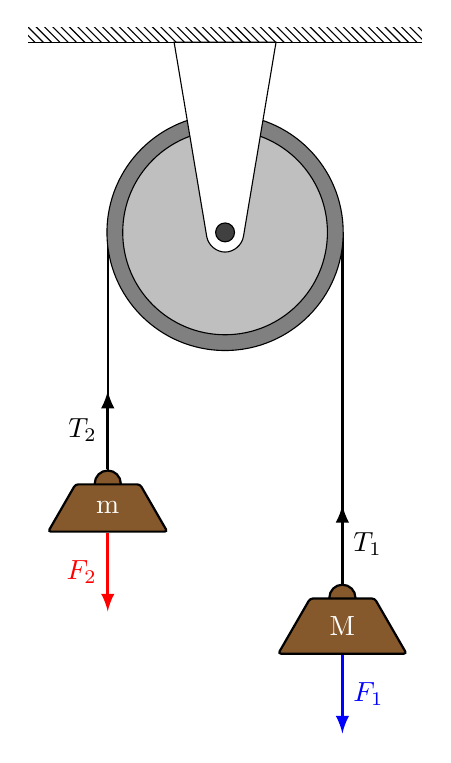
\begin{tikzpicture}

% Mass 1
\draw[thick] (1.49cm,0) -- ++(0,-5cm) node[draw=black,above=0.18cm,circle,fill=brown!70!black](cM){}
node[draw=black,trapezium,rounded corners=1pt,fill=brown!70!black,text=white, minimum height=0.7cm](M){M};

% Mass 2
\draw[thick] (-1.49cm,0) -- ++(0,-3.5cm) node[draw=black,above=0.13cm,circle,fill=brown!70!black](cm){} node[draw=black,trapezium,rounded corners=1pt,fill=brown!70!black,text=white, minimum height=0.6cm](m){m};

% Supporting structure
\fill[pattern= north west lines,] (-2.5,2.41) rectangle (2.5,2.6);
\draw(-2.5,2.41) -- (2.5,2.41);

% Pulley
\draw[fill = gray] (0,0) circle (1.5cm); % Big circle
\draw[fill=lightgray] (0,0) circle (1.3cm); % Medium circle
\draw[fill=white] (75:2.5) to[rounded corners=0.2cm] (0.2,-0.25) to[rounded corners=0.2cm] (-0.2,-0.25) -- (105:2.5) -- cycle;
\draw[fill=darkgray] (0,0) circle (0.12cm); % Axle circle

% Forces
\draw [-latex,very thick,blue] (M.bottom side) -- ++(0,-1) node[midway,right]{$F_1$};
\draw [-latex,very thick,black] (cM.north) -- ++(0,1)node[midway,right]{$T_1$};

\draw [-latex,very thick,red] (m.bottom side) -- ++(0,-1)node[midway,left]{$F_2$};
\draw [-latex,very thick,black] (cm.north) -- ++(0,1)node[midway,left]{$T_2$};

\end{tikzpicture}

\end{document}
